\scanpage{26}
\mspage{23}
II) $I\cap J\ne\{y\}$ \qquad Deux cas

\deleted{a) $\unsure{I\cap J=\{x,y\}}$}

\deleted{\figure{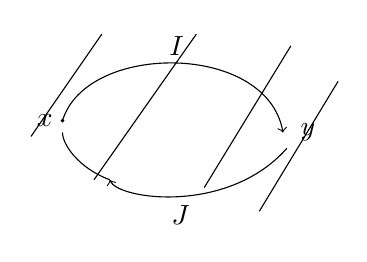
\begin{tikzpicture}[x=1cm,y=1cm]
\draw[->] (0,0) .. controls (.3,1) and (2.6,1) .. (2.8,-.15);
\draw[->] (2.85,-.35) .. controls (2.1,-1.2) and (.7,-1) .. (.6,-.75);
\draw (.6,-.75) .. controls (.2,-.6) and (0,-.3) .. (0,-.15);
\fill (0,0) circle(.025);
\node[left] at (0,0) {$x$}; \node[right] at (2.9,-.15) {$y$};
\node[above] at (1.45,.7) {$I$}; \node[below] at (1.5,-.95) {$J$};
\draw (-.4,-.2)--(.5,1.1); \draw (.4,-.75)--(1.7,1.1);
\draw (1.8,-.85)--(2.9,.95); \draw (2.5,-1.15)--(3.5,.5);
\end{tikzpicture}}}

\deleted{b) $x\ne y$}
Soit $w\in I\cap J$, $w\ne y$
et considérons
\[
\begin{array}{c}
\uline{J_{y,w}}\\[-.4ex]
\rotatebox{-90}{$\in$}\\[-.4ex]
S
\end{array}
\subset J,\quad \uline{I_{w,y}}
\]

\margin{\figure{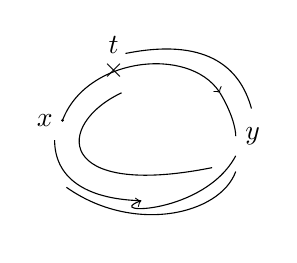
\begin{tikzpicture}[x=1cm,y=1cm]
\draw[->] (0,0) .. controls (.3,.8) and (1.6,.95) .. (2,.35);
\draw (2,.35) .. controls (2.15,.1) and (2.2,-.1) .. (2.2,-.2);
\draw[->] (2.2,-.45) .. controls (1.8,-1.2) and (.5,-1.2) .. (1,-1.02);
\draw (1,-1.02) .. controls (.25,-1) and (-.1,-.7) .. (-.1,-.25);
\draw (.8,.85) .. controls (1.8,1.05) and (2.25,.7) .. (2.4,.15);
\draw (.75,.35) .. controls (-.1,-.05) and (-.1,-1) .. (1.9,-.6);
\draw (.05,-.85) .. controls (.9,-1.45) and (2,-1.2) .. (2.2,-.65);
\fill (0,0) circle(.02); \node[left] at (0,0) {$x$};
\node[right] at (2.2,-.2) {$y$};
\node at (.65,.63) {$\times$}; \node[above] at (.65,.72) {$t$};
\end{tikzpicture}}}

\figure{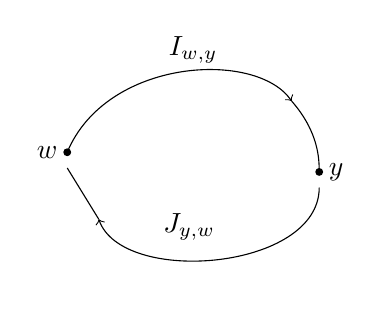
\begin{tikzpicture}[x=1cm,y=1cm]
\draw[->] (0,0) .. controls (.5,1.2) and (2.4,1.3) .. (2.85,.65);
\draw (2.85,.65) .. controls (3.2,.25) and (3.2,-.1) .. (3.2,-.25);
\draw[->] (3.2,-.45) .. controls (3.2,-1.5) and (.7,-1.7) .. (.4,-.85);
\draw (.4,-.85)--(0,-.2);
\fill (0,0) circle(.05); \fill (3.2,-.25) circle(.05);
\node[left] at (0,0) {$w$}; \node[right] at (3.2,-.25) {$y$};
\node[above] at (1.6,1) {$I_{w,y}$};
\node at (1.55,-.95) {$J_{y,w}$};
\end{tikzpicture}}

\margin{\uline{NB} $w$ régulier \uline{sauf} si \deleted{$w\in\{x,z\}$}
$w=x=z$ \deleted{\unsure{et}} i.e.
si on
\figure{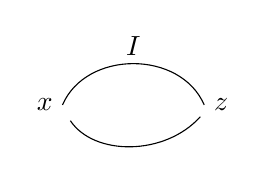
\begin{tikzpicture}[x=1cm,y=1cm]
\draw (0,0) .. controls (.3,.7) and (1.5,.7) .. (1.8,0);
\draw (.1,-.2) .. controls (.4,-.65) and (1.3,-.65) .. (1.75,-.15);
\node[left] at (0,0) {$x$}; \node[right] at (1.8,0) {$z$};
\node[above] at (.9,.5) {$I$};
\end{tikzpicture}}}

\deleted{Je dis que $I_{w,y}\cap$}

Je vais donc étudier d'abord la situation

\figure{\begin{tikzpicture}[x=1cm,y=1cm]
\draw[->] (0,0) .. controls (.2,1) and (1.3,1.4) .. (2.1,1.05);
\draw (2.1,1.05) .. controls (2.6,.8) and (2.9,.3) .. (3,0);
\draw[->] (3,-.25) .. controls (3,-1.8) and (.4,-1.7) .. (.1,-.4);
\draw[dashed] (1,1.08)--(1,-1.35);
\draw (0,0) circle(.035); \fill (3,0) circle(.05);
\fill (1,1.08) circle(.04); \fill (1,-1.35) circle(.04);
\node[left] at (0,0) {$x$}; \node[right] at (3,0) {$y$};
\node[above] at (1,1.08) {$t$}; \node[below] at (1,-1.35) {$t$};
\node[above] at (1.65,1.3) {$I$}; \node at (1.7,-1.05) {$J$};
\end{tikzpicture}}

\margin{$\operatorname{br}_y I\ne\operatorname{br}_y J$

\uline{NB} On ne va pas exiger $y$ régulier}

\deleted{$I\cap J\unsure{=}$}
\[
\delta I=\delta J,\quad I\cap J=?
\]
Je dis que $\operatorname{br}_x(I)\ne\operatorname{br}_x(J)$. Sinon,
en vertu de l'axiome F6, existerait $K\in S$, tel que :
$x\in\delta K$, et $I=K_{x,y}$, $J=K_{xy}$
donc $I=J$, donc $\operatorname{br}_y(I)=\operatorname{br}_y J$, absurde.

Je dis que $I\cap J=\{x,y\}$. Si on avait
$t\in I\cap J$, $t\notin\{x,y\}$, donc $t\in I^\circ\cap J^\circ$,
\unsure{en appliquant|on appliquerait} ce qui précède à $I_{x,t}$, $J_{x,t}$
\mspage{25}

\rotatebox{90}{\unsure{EXTRA STRONG}}
\rotatebox{90}{\unsure{EXTRA STRONG}}
